% 08_tungsten.tex -- Part 8, tungsten as a donor in crystalline In2O3. Sources: research_monograph/chapters/
% M10_w_and_vacancies.tex (sec:mono-w-cells, sec:mono-w-site, sec:mono-w-level, tab:mono-w-cells, tab:mono-w-open,
% keyresult), M06_defect_theory.tex (sec:mono-defect-hydrogenic, sec:mono-defect-resonant), M03_literature_materials.tex
% (sec:mono-lit-w), M08_c10_campaign.tex (tab:mono-c10-models: donors 2.5e17 V1 fitted, accumulation 5.6e19),
% 13_dft_rev.tex l.1231 (Shannon radius sums incl. W5+), appendices/MG_corrections.tex (X1, X7, X9, X11);
% evidence/FACT_REGISTRY.tsv (FACT-004, 005, 040-048, 080, 082); evidence/derived/defect_estimates.json;
% research_record/03_CLAIMS_LEDGER.yaml (C022); qe_workflow/cern_htcondor/results/RESULTS_LOG.md (2026-09-29,
% 2026-09-30, 2026-10-05 CORRECTION, 2026-10-14 C022 caveat); qe_workflow/analysis_2026-10-13_full/out/
% f09_iwo_bulk.json, f10_iwo_slabs.json. Figures: tools/fig_08_tungsten.py (data: f09/f10 JSON, raw bands.out of
% iwo_W8b and iwo_W24d, bands_masses/out/b01_masses.json). Crystalline cells only; no amorphous quantity appears.
% Note: frame bodies start with a command, never with a brace group (beamer would read a subtitle).
\partslide{Part 8}{Tungsten as a donor}

% denser slides: footnotesize bullets, local to the frame in which it is called
\providecommand{\eightdense}{\setbeamerfont{itemize/enumerate body}{size=\footnotesize}%
  \setbeamerfont{itemize/enumerate subbody}{size=\footnotesize}}
% pull the frame body up towards the title rule (as \fiveTop in Part 5)
\providecommand{\eightTop}{\vspace{-4mm}}

% ---------------------------------------------------------------------------------------------------------------------
\begin{frame}{W cells donate 1.4--3.0$\times10^{21}$\cmcu, far above the Mott density}
  \eightdense\eightTop
  \begingroup\scriptsize
  \renewcommand{\arraystretch}{1.02}
  \begin{tabularx}{\textwidth}{@{}X l c l c@{}}
    \toprule
    cell & composition & W / cations & W site & donated density \\
    \midrule
    bulk, 80 atoms, PBE lattice $a = 10.3061$\,\AA & In$_{31}$WO$_{48}$ & 3.1\,\% & 24d or 8b & $2.7\times10^{21}$\cmcu \\
    relaxed 1\,nm film & In$_{23}$WO$_{48}$H$_{24}$ & 4.2\,\% & central 24d & $3.0\times10^{21}$\cmcu \\
    relaxed 2\,nm film & In$_{55}$WO$_{96}$H$_{24}$ & 1.8\,\% & central 24d & $1.4\times10^{21}$\cmcu \\
    \bottomrule
  \end{tabularx}\par\endgroup
  \src{PAW-PBE, 71/568\,Ry; Marzari--Vanderbilt (MV) smearing 0.01\,Ry; ions relaxed at fixed cell (bulk on
    3$\times$3$\times$3, final SCF on 4$\times$4$\times$4); claim C022; this work \lab{computed}.}
  \begin{columns}[T,onlytextwidth]
    \begin{column}{0.53\textwidth}
      \begin{itemize}
        \item The device paper credits W with ``smoother charge delocalization''\sref[p.~4]{Januar2026}. Here: where
          the W level lies and where its electrons go.
        \item Hydrogenic donor: $E_D \approx 25$\,meV, Mott density $n_c \approx 9\times10^{17}$\cmcu{} \lab{derived}
          (Part~12; derivation in backup).
        \item Device model (Part~4, open circles): donors below $n_c$ \lab{fitted}; on-state channel (2\,nm film, 2\,V
          overdrive) degenerate \lab{derived}.
      \end{itemize}
    \end{column}
    \begin{column}{0.44\textwidth}
      \centering
      \begin{tikzpicture}[x=1mm,y=1mm,font=\scriptsize,line width=0.5pt]
        % log axis 1e17 .. 1e22, 11 mm per decade
        \draw (0,0) -- (55,0);
        \foreach \e/\x in {17/0,18/11,19/22,20/33,21/44,22/55} {
          \draw (\x,0) -- (\x,1.2);
          \node[anchor=north,inner sep=1.2pt] at (\x,0) {$10^{\e}$};
        }
        \node[anchor=north] at (27.5,-4.0) {electron density (cm$^{-3}$)};
        % Mott density 9.1e17: log10 = 17.96 -> 10.54 mm
        \draw (10.54,0) -- (10.54,10.5);
        \node[anchor=south,align=center] at (10.54,10.5) {Mott density $n_c$\\[-0.3mm]$9\times10^{17}$};
        % W cells 1.4e21 .. 3.0e21: log10 = 21.146 .. 21.477 -> 45.6 .. 49.2 mm
        \draw[line width=2.4pt] (45.6,3.2) -- (49.2,3.2);
        \draw (45.6,0) -- (45.6,3.2);
        \draw (49.2,0) -- (49.2,3.2);
        \draw[rulegrey] (47.4,4.4) -- (47.4,10.5);
        \node[anchor=south,align=center] at (47.4,10.5) {W cells\\[-0.3mm]1.4--3.0$\times10^{21}$};
        \draw[{Stealth[length=1.6mm]}-{Stealth[length=1.6mm]},ntumaroon,line width=0.7pt] (11.3,6.6) -- (44.8,6.6);
        \node[anchor=south,ntumaroon] at (28,6.9) {1500--3300 times};
        % device model (M08): donors 2.5e17 -> 17.398 -> 4.38 mm; on-state 5.6e19 -> 19.748 -> 30.23 mm
        \draw[fill=white] (4.38,0) circle (0.75mm);
        \node[anchor=south,align=center,inner sep=1pt] at (4.0,1.0) {donors\\[-0.6mm]$2.5\times10^{17}$};
        \draw[fill=white] (30.23,0) circle (0.75mm);
        \node[anchor=south,inner sep=1pt] at (30.23,1.0) {on-state $5.6\times10^{19}$};
      \end{tikzpicture}
      \src{W cells: 3\,e per W (formal count) per cell volume (films: H--H thickness) \lab{derived}.
        Device model: donors \lab{fitted}; on-state \lab{derived}.}
    \end{column}
  \end{columns}
  \takeaway{The cells hold no bound hydrogenic state; they locate the W-5d level in the band.}
\end{frame}

% ---------------------------------------------------------------------------------------------------------------------
\begin{frame}{W prefers 24d by 0.258\,eV; W--O bonds consistent with W$^{6+}$}
  \eightdense\eightTop
  \begin{columns}[T,onlytextwidth]
    \begin{column}{0.42\textwidth}
      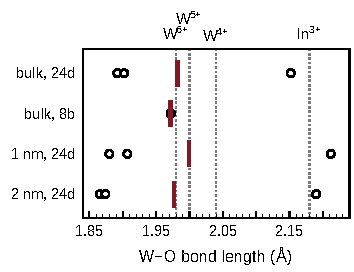
\includegraphics[width=\linewidth]{08_bonds}
      \src{W--O bonds of the relaxed cells (circles; each value occurs twice on 24d, six times on 8b); bars: mean
        bond; dotted: Shannon radius sums for six-fold cations with O$^{2-}$ (1.38\,\AA). This
        work, PAW-PBE \lab{computed}.}
    \end{column}
    \begin{column}{0.55\textwidth}
      \begin{itemize}
        \item $\Delta E = E(\mathrm{8b}) - E(\mathrm{24d}) = 0.2579$\,eV (3$\times$3$\times$3 relaxation),
          0.2577\,eV (4$\times$4$\times$4) \lab{computed}.
        \item Three 24d sites per 8b site: $N_{\mathrm{24d}}/N_{\mathrm{8b}} = 3\exp(\Delta E/\kT) \approx 440$ at
          600\,K; 8b is practically empty at any processing temperature \lab{derived}.
        \item Mean W--O bond: bulk 1.982 (24d), 1.972\,\AA{} (8b); films 2.000 (1\,nm), 1.977\,\AA{} (2\,nm)
          \lab{computed}. Shannon sums\sref{Shannon1976}: 1.98 (W$^{6+}$), 2.00 (W$^{5+}$), 2.04\,\AA{} (W$^{4+}$).
        \item Bulk and 2\,nm means are consistent with W$^{6+}$; the 1\,nm mean sits at the W$^{5+}$ sum. An ionic-radius argument,
          not a charge measurement (record correction X11).
      \end{itemize}
    \end{column}
  \end{columns}
  \takeaway{W sits on 24d; formally W$^{6+}$, it leaves three electrons per W above the valence band.}
\end{frame}

% ---------------------------------------------------------------------------------------------------------------------
\begin{frame}{At 3\,e per cell the W-5d-rich state lies 1.2--1.8\,eV above $\Ec$}
  \eightdense\eightTop
  \begin{columns}[T,onlytextwidth]
    \begin{column}{0.42\textwidth}
      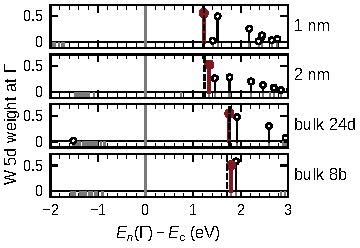
\includegraphics[width=\linewidth]{08_levels}
      \src{W-5d weight of each state at $\Gamma$ against its energy relative to the host conduction-band bottom $\Ec$; grey
        ticks: all states; dashed: $\EF$; maroon: $E_{\mathrm{W}}$, the first state above the host-band bottom with
        W 5d $\ge 0.3$ at $\Gamma$; in bulk 8b a state 0.10\,eV higher has 58\,\%. PBE, MV 0.01\,Ry. This work
        \lab{computed}.}
    \end{column}
    \begin{column}{0.55\textwidth}
      \begingroup\scriptsize
      \renewcommand{\arraystretch}{1.05}
      \begin{tabular*}{\linewidth}{@{\extracolsep{\fill}}l c c c@{}}
        \toprule
        cell (W site) & $\EF - \Ec$ & $E_{\mathrm{W}} - \Ec$ & $E_{\mathrm{W}} - \EF$ \\
        \midrule
        1\,nm film (24d) & 1.228 & 1.22 & $-0.005$ \\
        2\,nm film (24d) & 1.238 & 1.34 & $+0.103$ \\
        bulk (24d) & 1.763 & 1.76 & $+0.001$ \\
        bulk (8b) & 1.713 & 1.80 & $+0.090$ \\
        \bottomrule
      \end{tabular*}\par\endgroup
      \src{Energies in eV at $\Gamma$, at the computed filling (3\,e per cell, 1.4--3.0$\times10^{21}$\cmcu);
        $E_{\mathrm{W}}$: W-5d-rich level. Claim C022 \lab{computed}.}
      \begin{itemize}
        \item Resonant donor\sref{Swallow2020}: a level inside the band hybridises with it; the donor is ionised at
          any temperature, and the level fills only once $\EF$ reaches it \lab{theory}.
        \item In every cell a W-5d-rich state (50--60\,\% W 5d at $\Gamma$) lies 1.22--1.80\,eV above $\Ec$, within
          about 0.1\,eV of $\EF$ \lab{computed}.
        \item Not proof of pinning: a partly filled narrow level sits at $\EF$ by construction; 0.1\,eV is below the
          0.136\,eV smearing.
      \end{itemize}
    \end{column}
  \end{columns}
  \takeaway{At the cells' filling, $\EF$ has risen through the host band up to the W resonance.}
\end{frame}

% ---------------------------------------------------------------------------------------------------------------------
\begin{frame}{Most donated electrons fill the host band, not the W level}
  \eightdense\eightTop
  \begin{columns}[T,onlytextwidth]
    \begin{column}{0.40\textwidth}
      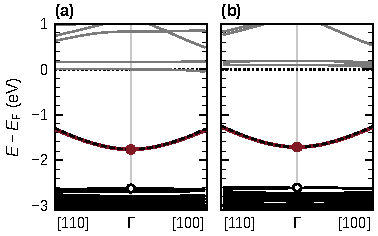
\includegraphics[width=\linewidth]{08_bands}
      \src{Bulk W cells, (a) 24d, (b) 8b. Black: valence bands (circle: top, band 351); maroon: host conduction band
        (352); grey: W-5d-rich and folded host bands; dashed: pure-bulk band shifted to the host minimum (nearly on
        the maroon curve: masses differ by 5\,\%); dotted: $\EF$. This work \lab{computed}.}
    \end{column}
    \begin{column}{0.57\textwidth}
      \begin{itemize}
        \item Of three electrons, the lowest host band holds 1.79 (24d), 1.93 (8b), 2.00 (1\,nm); the W-5d-rich band
          (half W 5d at $\Gamma$) 1.13, 0.95, 0.99 \lab{computed}.
        \item Kane band\sref{Kane1957} filled to the computed $\EF$:\vspace{-1.5mm}
          \[ N = \frac{\Omega\,k_F^3}{3\pi^2}, \quad \frac{\hbar^2k_F^2}{2m_b} = E(1+\alpha E), \quad E = \EF-\Ec \]
          \vspace{-3.8mm}\par
          $N$: electrons per cell, $k_F$: Fermi wave vector; $\Omega = 1094.6$\,\AA$^3$, $m_b = 0.162\,m_0$,
          $\alpha = 0.58$\,eV$^{-1}$ give 2.17 (24d), 2.04\,e (8b), above the computed 1.79, 1.93; a parabolic band
          gives 0.76, 0.73\,e \lab{derived}.
        \item W makes the bulk host band 5\,\% heavier (0.162 vs 0.1541\,$m_0$) and narrows the film gaps by 0.069
          (1\,nm), 0.148\,eV (2\,nm) \lab{computed}: consistent with band-gap renormalisation\sref{Hamberg1986}
          \lab{inferred}; strain not separated.
      \end{itemize}
    \end{column}
  \end{columns}
  \takeaway{A non-parabolic host band can hold two electrons per cell; a parabolic one cannot.}
\end{frame}

% ---------------------------------------------------------------------------------------------------------------------
\begin{frame}{Record correction X1: the ``deep W level'' was a band miscount}
  \eightdense\eightTop
  \begin{columns}[T,onlytextwidth]
    \begin{column}{0.52\textwidth}
      \centering
      \begin{tikzpicture}[x=0.89mm,y=10.5mm,font=\scriptsize,line width=0.5pt]
        % energy axis: E - E_F at Gamma (eV), 1 nm W film; levels: f10_iwo_slabs.json, bands 311-314
        \draw (0,-3.1) -- (0,0.4);
        \foreach \v in {-3,-2,-1,0} { \draw (0,\v) -- (1.2,\v); \node[anchor=east,inner sep=1.5pt] at (0,\v) {$\v$}; }
        \node[rotate=90,anchor=south,inner sep=1pt] at (-4.6,-1.35) {$E - \EF$ at $\Gamma$ (eV)};
        \draw[dashed] (2.5,0) -- (70,0);
        % column headers
        \node[anchor=south] at (15,0.5) {\textbf{30 Sep reading}};
        \node[anchor=south] at (50,0.5) {\textbf{corrected, 5 Oct}};
        % superseded reading
        \draw[rulegrey,line width=1pt] (3,-2.947) -- (13,-2.947);
        \node[anchor=west,inkgrey] at (14,-2.947) {311};
        \draw[line width=1pt] (3,-1.228) -- (13,-1.228);
        \node[anchor=west] at (14,-1.228) {``VB top'' (312)};
        \draw[ntumaroon,line width=1.4pt] (3,-0.005) -- (13,-0.005);
        \draw[line width=1pt] (3,0.185) -- (13,0.185);
        \node[anchor=west] at (14,0.30) {``CB bottom'' (314)};
        \node[anchor=north west,ntumaroon,align=left,inner sep=1pt] at (14,-0.06) {``W level'' (313),\\[-0.4mm]0.19\,eV below ``CB''};
        \node[anchor=west,inkgrey] at (3,-0.75) {``gap'' 1.22\,eV};
        % corrected reading
        \draw[line width=1pt] (41,-2.947) -- (51,-2.947);
        \node[anchor=west,align=left] at (52,-2.947) {VB top\\[-0.4mm]311: O 2p};
        \draw[line width=1pt] (41,-1.228) -- (51,-1.228);
        \node[anchor=west,align=left] at (52,-1.228) {host CB bottom\\[-0.4mm]312: In 5s 0.50};
        \draw[ntumaroon,line width=1.4pt] (41,-0.005) -- (51,-0.005);
        \node[anchor=north west,ntumaroon,align=left,inner sep=1pt] at (52,-0.06) {W-5d-rich\\[-0.4mm]313: W 5d 0.56};
        \draw[line width=1pt] (41,0.185) -- (51,0.185);
        \node[anchor=west] at (52,0.30) {314: host CB};
        \draw[{Stealth[length=1.6mm]}-{Stealth[length=1.6mm]},ntumaroon,line width=0.7pt] (46,-1.17) -- (46,-0.07);
        \node[anchor=west,ntumaroon] at (46.5,-0.71) {1.22\,eV};
        \draw[{Stealth[length=1.6mm]}-{Stealth[length=1.6mm]},line width=0.5pt] (39.5,-2.89) -- (39.5,-1.29);
        \node[anchor=east,align=right] at (39,-2.09) {gap\\[-0.4mm]1.72\,eV};
      \end{tikzpicture}
      \src{1\,nm W film, eigenvalues at $\Gamma$; dashed: $\EF$; character from projections (fraction of the state).
        Data: project results log, 30 Sep and 5 Oct 2026; claim C022; this work \lab{computed}.}
    \end{column}
    \begin{column}{0.45\textwidth}
      \begin{itemize}
        \item Cause: the band-count rule of the PAW data sets (Part~5); here band 311 is the VB top and band 312 the
          host CB bottom.
        \item Reading band 312 as the VB top put a W level 0.19\,eV below the host CB (band 314), $\EF$ pinned in it
          (a deep donor), and a 1.1--1.65\,eV vacuum-scale shift: both artefacts.
        \item Projections at $\Gamma$ fix each band: corrected 5 Oct, refined 14 Oct.
        \item The false reading would have fitted the device data well \lab{inferred}; withdrawn, kept in the record.
      \end{itemize}
    \end{column}
  \end{columns}
  \takeaway{At the computed filling W is a resonant donor 1.2--1.8\,eV above $\Ec$, not a deep level.}
\end{frame}

% ---------------------------------------------------------------------------------------------------------------------
\begin{frame}{W donates into the host band; ionisation in devices is inferred}
  \eightdense\eightTop
  \begingroup\scriptsize
  \renewcommand{\arraystretch}{1.06}
  \begin{tabularx}{\textwidth}{@{}>{\raggedright\arraybackslash}p{6.3cm} >{\raggedright\arraybackslash}p{1.55cm}
      >{\raggedright\arraybackslash}X@{}}
    \toprule
    statement & status & basis, or the calculation that would decide \\
    \midrule
    W donates; the host band holds most of the electrons & \leavevmode\lab{computed} & four cells,
      1.4--3.0$\times10^{21}$\cmcu, one filling each \\
    W-5d-rich level 1.2--1.8\,eV above $\Ec$, within 0.1\,eV of $\EF$ & \leavevmode\lab{computed} & PBE only;
      no hybrid functional for the W cells \\
    The resonance pins $\EF$ & \leavevmode\lab{hypothesis} & needs a density series: 160-atom cell, one W (1.6\,\%) \\
    W stays ionised at device densities ($\EF$ below $\Ec$) & \leavevmode\lab{inferred} & needs the 160-atom cell and
      HSE06 on the 80-atom cell (amendment A23(ii)); a hybrid may lower the d level \\
    W may trap an electron as a polaron (not computed) & \leavevmode\lab{hypothesis} & symmetry-broken PBE+$U$ or
      HSE06 starts \\
    Spin moments 0.62 (24d), 0.74\,$\mu_B$ (8b) per cell & \leavevmode\lab{computed} &
      3$\times$3$\times$3, preliminary, not claimed: likely spurious Stoner moments (record correction X7) \\
    \bottomrule
  \end{tabularx}\par\endgroup
  \vspace{0.5mm}
  \begin{itemize}
    \item If the W level stays $\ge 1.2$\,eV above $\Ec$ at device densities (not computed), its occupation for
      $\EF \le \Ec$ is below $\exp(-1.2\,\mathrm{eV}/\kT) \approx 10^{-20}$ at 300\,K \lab{derived}.
    \item Mo 4d states lie high in the conduction band of \InO{} (photoemission, hybrid DFT), and the ionised donor
      scatters less\sref{Swallow2020}; for W this is an analogy \lab{inferred}.
  \end{itemize}
  \takeaway{W is a resonant donor at the computed filling; lower densities remain untested.}
\end{frame}
